\documentclass[fleqn]{article}
\usepackage[left=1in, right=1in, top=1in, bottom=1in]{geometry}
\usepackage{mathexam}
\usepackage{graphicx}

\ExamClass{CSCE 240}
\ExamName{Homework 5}
\ExamHead{Due: 05 November 2018}

\let
\ds
\displaystyle

\begin{document}
\ExamInstrBox {
You shall upload a zipped (AND ONLY ZIPPED) archive to Blackboard containing the
directory hw5 and:
\begin{enumerate}
  \item A \texttt{hw5/vector2d.h} file with your includes and class declarations,
  \item A \texttt{hw5/vector2d.cc} file with your class definitions,
  \item A \texttt{hw5/point2d.h} file with your includes and class declarations,
        and
  \item A \texttt{hw5/point2d.cc} file with your class definitions, at least.
\end{enumerate}
}
\vspace{1.0em}

We are creating a more C++-like library. We are implementing a pair of
classes---Point2d and Vector2d. These classes implement the behavior of
two-dimensional points and vectors in a Cartesian coordinate system.
\\

They are described in the UML below as well the attached header files.
%
\begin{center}
	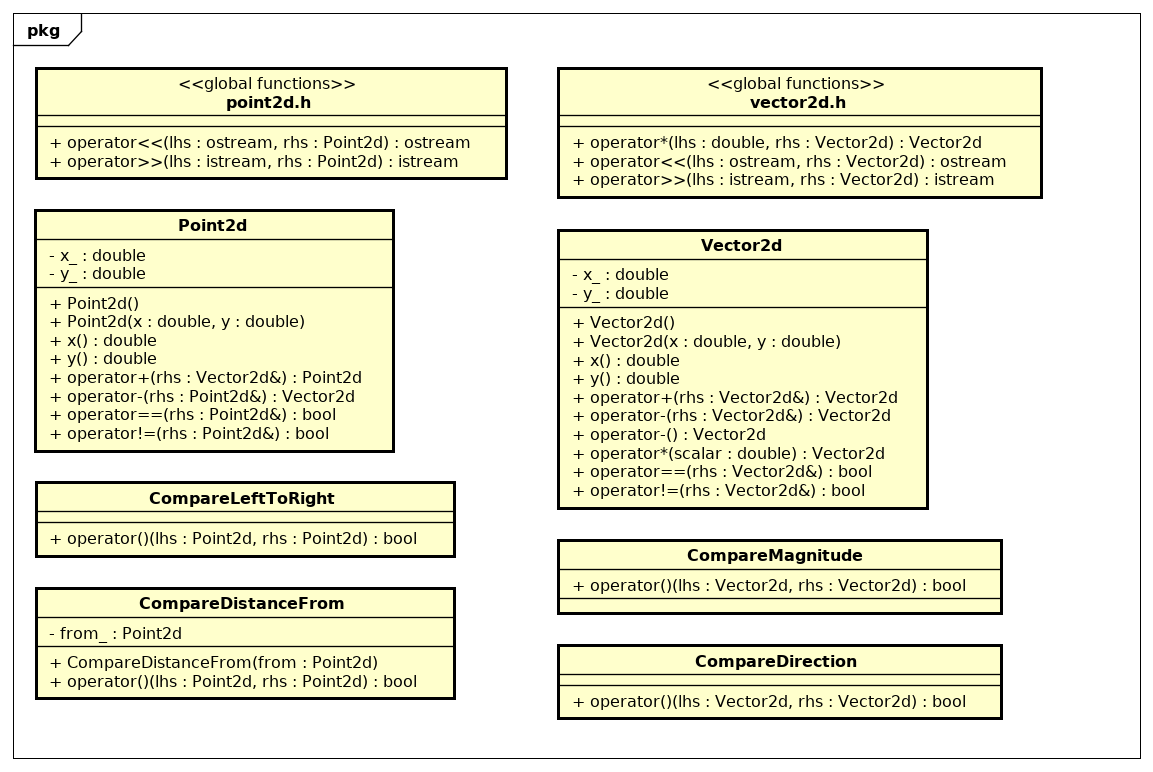
\includegraphics[width=0.75\columnwidth]{hw5}
\end{center}
%

In an effort to force you to read others' code, I have provided you with a
fairly detailed set of unit test functions demonstrating the functionality. IJ
and I will be referring any questions answered by reading the provided Unit
Tests to the provided Unit Tests. Questions about the tests themselves or
beyond the tests will, of course, be answered.
\\

You may compile and link to them to ensure that your classes meet all
requirements. The behavior demonstrated in the tests should well-define the
expectations of the classes' operations.
\newpage
%
The libraries are further described as follows:
\begin{enumerate}
  \item vector2d.h
  \begin{enumerate}
    \item Vector2d---a two-tuple representing direction and magnitude in the
    Cartesian coordinate system.
    \begin{enumerate}
      \item operator+ and operator- return the result of the operation where
        the calling object is the left-hand side of the operation
      \item operator- returns a vector with the opposite direction of calling
        object
      \item operator== and operator!= return true or false when approximately
        equal or not 
    \end{enumerate}

    \item global functions
      \begin{enumerate}
        \item \texttt{operator*} return the result of scaling the rhs by the
        lhs
        \item \texttt{operator$<<$} extracts a vector of the form (1.0, 2.0)
        into the ostream, where 1.0 and 2.0 are the member variables.
        \item \texttt{operator$>>$} inserts into the rhs, from the istream in
        the form "1.0 2.0"
      \end{enumerate}

    \item CompareMagnitude---overloads the \texttt{operator()} operator such
    that it returns true if lhs has less magnitude than rhs, false otherwise
    \item CompareDirection---overloads the \texttt{operator()} operator such
    that it returns true if lhs is closer to 0 than rhs when converted to
    angles. You may use \texttt{atan2} from cmath, but keep in mind that it
    provides a range from $[-\pi, \pi]$ and the range we want to simulate is
    $[0.0, 2\pi)$ 
  \end{enumerate}

  \item point2d.h
    \begin{enumerate}
      \item Point2d---a two-tuple representing location in the Cartesian
      coordinate system.
      \begin{enumerate}
        \item operator- returns the magnitude and direction from the calling
          object to the Point2d parameter as a Vector2d
        \item operator+ returns a Point2d offset from the calling object by the
          Vector2d parameter
        \item operator== and operator!= return true if approximately equal or
        not
      \end{enumerate}

      \item global functions
        \begin{enumerate}
          \item operator$<<$ extracts the values from the calling object as $(x,
            y)$ and adds to the ostream parameter, then returns the ostream
            parameter
          \item operator$>>$ reads two floating point values from the istream
            and adds them to the two attributes of the calling object, then
            returns the istream parameter.
        \end{enumerate}
      \item CompareLeftToRight---overloads the \texttt{operator()} operator and
        returns true when lhs has a lesser x coordinate or if equal in x, a
        lesser y coordinate.
      \item CompareDistanceFrom---overloads the \texttt{operator()} operator and
        returns true when lhs is closer to the point stored in the constructor
        than rhs.
    \end{enumerate}
\end{enumerate}

As in the previous assignments, you will receive up to 100\% credit for turning
it on the day it is due and will lose 25\% per day late.
\\

There are 7 points possible in the tests and another 3 possible in the
styling. 

\end{document}

